\documentclass[a4paper,10pt]{article}
\usepackage{fullpage}
\usepackage{mathtools}
\usepackage{bm}
\usepackage{graphicx}

\title{DIALS Integration Processing}
\author{James Parkhurst}

\begin{document}

\maketitle

\section{Source code}

The source code for everything I've done so far can be found in the dials 
sourceforge repository at /dials-code/scratch/jmp/extract\_reflection\_profiles.

\section{Coordinate Systems and parameters}

\noindent
The following coordinate systems are used:

\begin{itemize}
  \item The laboratory system,         $\{\bm{l}_1,   \bm{l}_2,   \bm{l}_3  \}$.
  \item The detector system,           $\{\bm{d}_1,   \bm{d}_2,   \bm{d}_3  \}$.
  \item The goniostat system,          $\{\bm{m}_1,   \bm{m}_2,   \bm{m}_3  \}$.
  \item The crystal system,            $\{\bm{b}_1,   \bm{b}_2,   \bm{b}_3  \}$.
  \item The reciprocal lattice system, $\{\bm{b}_1^*, \bm{b}_2^*, \bm{b}_3^*\}$.
  \item The profile specific system,   $\{\bm{e}_1,   \bm{e}_2,   \bm{e}_3  \}$
\end{itemize}

\noindent
The following parameters are used:

\begin{itemize}
  \item The miller indices of a lattice point, $\bm{h} = (h, k, l)$.
  \item The wavelength of the incident radiation, $\lambda$.
  \item The incident beam vector, $\bm{S}_0$. 
  \item The diffracted beam vector, $\bm{S}_1$.
  \item The unrotated reciprocal lattice vector, $\bm{p}_0^*$. 
  \item The rotated reciprocal lattice vector, $\bm{p}^*$.
  \item The distance from the crystal to the detector, $F$.
  \item The detector origin, $(X_0, Y_0)$.
  \item The starting image frame $Z_0$.
  \item The coordinate of a reflection in the image volume $(X, Y, Z)$.
  \item The starting rotation angle, $\phi _0$.
  \item The rotation angle of a reflection, $\phi$.
  \item The oscillation range, $\Delta \phi$.
  \item The initial crystal rotation matrix, $\bm{U}$.
  \item The orthogonalisation matrix, $\bm{B}$.
  \item The x and y detector pixel sizes, $d_{s,x}$ and $d_{s,y}$
  \item The rotation by $\phi$ around axis $\bm{m}_2$, $\bm{R}$.
\end{itemize}

\noindent
The matrix, $\bm{U} \bm{B}$ is related to the reciprocal lattice coordinate
system, $\{\bm{b}_1^*, \bm{b}_2^*, \bm{b}_3^*\}$,  as follows:

\begin{equation}
  \bm{U} \bm{B} = 
    \begin{pmatrix}
        b_{1,1}^* & b_{1,2}^* & b_{1,3}^* \\
        b_{2,1}^* & b_{2,2}^* & b_{2,3}^* \\
        b_{3,1}^* & b_{3,2}^* & b_{3,3}^* \\ 
    \end{pmatrix}
  \label{ub-b* relation}
\end{equation}


\noindent
The components of the goniometer coordinate system, 
$\{\bm{m}_1,   \bm{m}_2,   \bm{m}_3  \}$, can be calculated from $\bm{m}_2$, 
the rotation axis, and $\bm{S}_0$, the incident beam vector, as follows:

\begin{equation}
  \begin{aligned}
    \bm{m}_1 &= (\bm{m}_2 \times \bm{S}_0) / |\bm{m}_2 \times \bm{S}_0| \\
    \bm{m}_3 &= (\bm{m}_1 \times \bm{m}_2)
  \end{aligned}
\end{equation}

\noindent
The laboratory coordinate of a point on the detector specified by its pixel
coordinates can be found as follows:

\begin{equation}
  \bm{q} = (X - X_0) \bm{d}_1 + (Y - Y_0) \bm{d}_2 + F \bm{d}_3 
  \label{detector point}
\end{equation}


\section{Spot Prediction}

Given a set of miller indices, $\bm{h} = (h, k, l)$ and predicted rotation 
angles $\phi$, the positions of the reflections as recorded on the detector 
can be predicted. This can be done by calculating the reciprocal lattice vector, 
$\bm{p}_0^*$ of each point and by rotating the vector by the angle, $\phi$, 
about the rotation axis, $\bm{m}_2$.

\begin{align*}
  \bm{p}_0^* &= h \bm{b}_1^* + k \bm{b}_2^* + l \bm{b}_3^* \\
  \bm{p}^* &= \bm{R}(\bm{m}_2, \phi) \bm{p}_0^* \\
  \intertext{or given equation \refeq{ub-b* relation}}
  \bm{p}^* &= \bm{R}(\bm{m}_2, \phi) \bm{U} \bm{B} \bm{h}
\end{align*}

The diffracted beam vector can then be calculated as follows. 

\begin{equation}
  \bm{S}_1 = \bm{S}_0 + \bm{p}^* 
\end{equation}

For the reflection to be in the diffracting condition, the reciprocal lattice
point needs to be touching the surface of the Ewald sphere. For this to be the
case, $|\bm{S}_1| = |\bm{S}_0| = 1 / \lambda$.

Having calculated the diffracted beam vector, $\bm{S}_1$, the predicted position
of the spot on the detector can be calculated by finding the intersection of the
line, $\bm{q} = d \bm{S}_1$, starting at the origin of the laboratory coordinate 
system and the detector plane, $(\bm{q} - \bm{q}_0) \cdot \bm{d}_3$. Setting
$\bm{q}_0 = F \bm{d}_3$, the origin of the detector plane, the intersection
point $\bm{q}$ can be found by the following.

\begin{equation}
  \bm{q} = d \cdot \bm{S}_1 = \frac{F \bm{S}_1} {\bm{S}_1 \cdot \bm{d}_3} 
  \nonumber
\end{equation}

Having found the point, $\bm{q}$, in laboratory coordinates, where the spot 
should be recording on the detector plane, the detector pixel coordinates of the 
point can now be found. Subtract the detector origin from the intersection point 
of the diffracted beam vector and the detector plane; then calculate the 
distance along the detector $\bm{d1}$ axis of the resulting vector using 
scalar projection. Multiplying this by $|\bm{d}_1|$ rescales the value into
pixel coordinates.

\begin{equation}
  \left(\frac{F \bm{S}_1} {\bm{S}_1 \cdot \bm{d}_3} - F \bm{d}_3 \right) 
    \cdot \bm{d}_1 = X - X_0 
  \nonumber
\end{equation}

The same can be done for the detector $\bm{d}_2$ axis. If 
$F \bm{S}_1 \cdot \bm{d}_3 > 0$, the equations can be rearranged to calculate
the detector pixel coordinates as follows.

\begin{equation}
  \begin{aligned}
    X &= X_0 + F \bm{S}_1 \cdot \bm{d}_1 / \bm{S}_1 \cdot \bm{d}_3 \\
    Y &= Y_0 + F \bm{S}_1 \cdot \bm{d}_2 / \bm{S}_1 \cdot \bm{d}_3
  \end{aligned}
\end{equation}

The data is collected for several difference angles around the rotation axis.
This results in an image volume as shown in Figure \ref{image volume}. For each
reflection, the position in this image volume is given by the calculated
$(X, Y)$ pixel coordinate and frame number, $Z$, derived from the predicted 
rotation angle $\phi$ for the reflection.

\begin{figure}
  \centering
  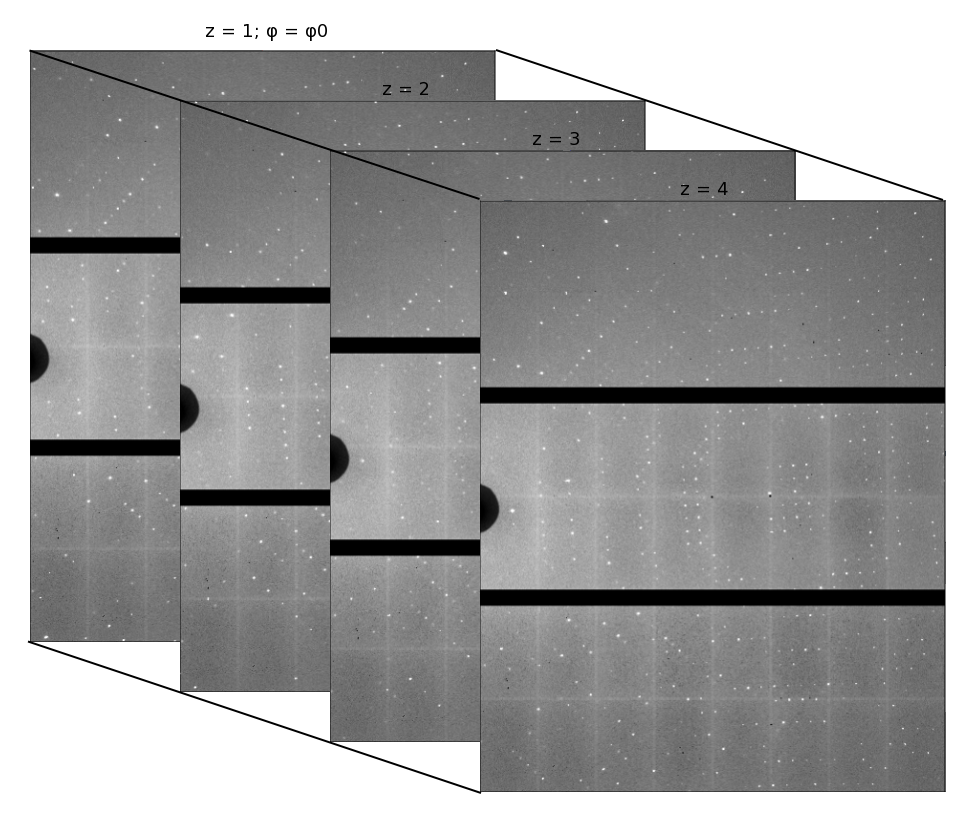
\includegraphics[width=0.66\textwidth]{./Figures/image_volume.png}
  \caption{The 3D image volume with each image captured at a different rotation 
    angle, $\phi'$}
  \label{image volume}
\end{figure}

Figure \ref{figure: spot prediction} shows the position of predicted spots on
three consecutive detectors images and a zoomed in view of the predicted 
positions.

\begin{figure}
  \centering
  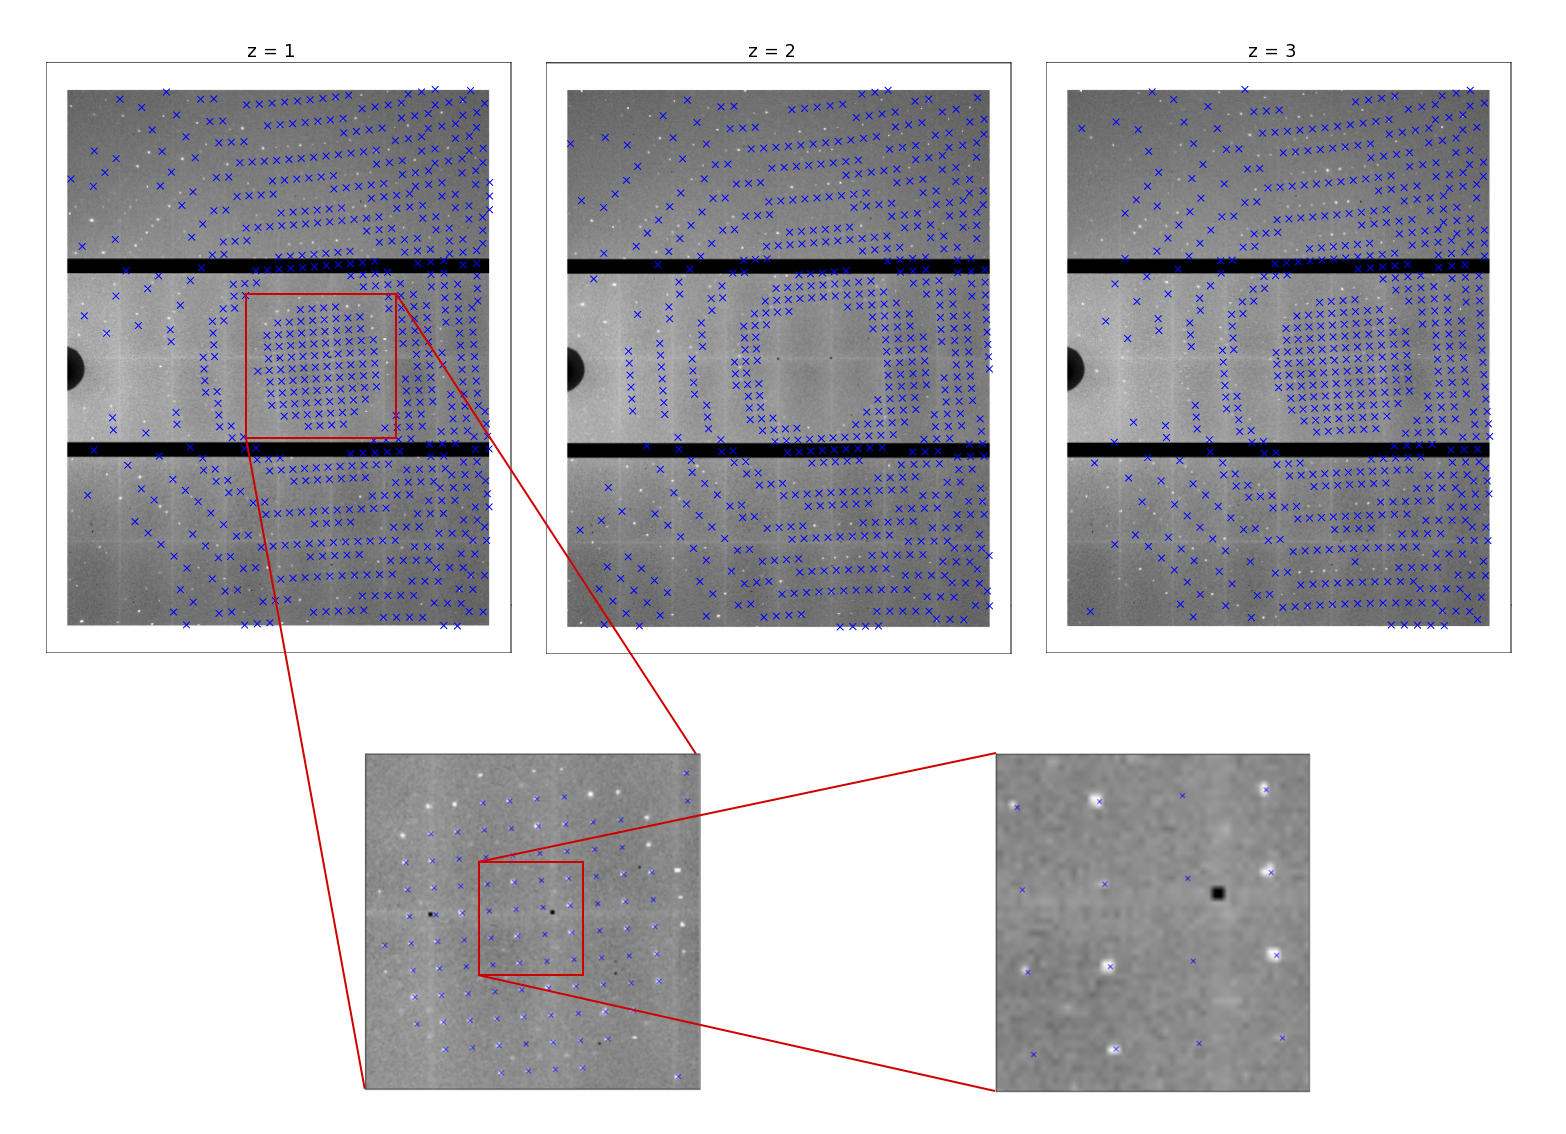
\includegraphics[width=0.66\textwidth]{./Figures/spot_prediction.png}
  \caption{Detector image showing the predicted position of spots.}
  \label{figure: spot prediction}
\end{figure}

\section{XDS Transform}

Now we have the $(X, Y, Z)$ coordinate of each reflection in the image volume.
In order to record each reflection with a standard spot shape, the detector
pixel values are transformed from the detector coordinate system to a coordinate
system specific to each reflection. The axes of the coordinate system are
defined as follows.

\begin{equation}
  \begin{aligned}
    \bm{e}_1 &= \bm{S}_1 \times \bm{S}_0 / |\bm{S}_1 \times \bm{S}_0| \\
    \bm{e}_2 &= \bm{S}_1 \times \bm{e}_1 / |\bm{S}_1 \times \bm{e}_1| \\
    \bm{e}_3 &= (\bm{S}_1 + \bm{S}_0)    / |\bm{S}_1 + \bm{S}_0|
  \end{aligned}
\end{equation}

For a given reflection, the coordinate system is defined as having it's origin 
at the point where the predicted $\bm{S}_1$ vector exits the Ewald sphere. The
coordinate system, $\{\bm{e}_1, \bm{e}_2, \bm{e}_3\}$, is defined such that
$\bm{e}_1$ is orthogonal to both $\bm{S}_0$ and $\bm{S}_1$, $\bm{e}_2$ is 
orthogonal to both $\bm{S}_1$ and $\bm{e}_1$ and $\bm{e}_3$ is orthogonal to
both $\bm{e}_1$ and $\bm{p}^* = \bm{S}_1 - \bm{S}_0$. $\bm{e}_1$ and $\bm{e}_2$
are, thus, tangents on the surface of the Ewald sphere. $\bm{e}_3$ represents
the velocity vector of the reflection as it passes through the Ewald sphere.

The pixel values are then mapped to the reflection coordinate system in the
following way. Taking a point $(X', Y')$ in the viscinity of the reflection
centre $(X, Y)$, the diffracted beam vector at that point is calculated using
equation \eqref{detector point} as follows.

\begin{equation}
  \begin{aligned}
    \bm{q}' = (X' - X_0) \bm{d}_1 + (Y' - Y_0) \bm{d}_2 + F \bm{d}_3, &\qquad
    \bm{S}' = \frac{\bm{q}'}{\lambda \cdot |\bm{q}'|}
  \end{aligned}
  \nonumber
\end{equation}

The coordinates are then calculated using the following equations. A scale
factor of $180 / (\pi |\bm{S}_1|)$ is used to scale the coordinates to degrees
($|\bm{S}_1| = 1 / \lambda$, the radius of the Ewald sphere).

\begin{equation}
  \begin{aligned}
    C_1        &= 180 / (\pi |\bm{S}_1|)\\
    C_2        &= 180 / (\pi |\bm{p}^*|)\\
    \epsilon_1 &= \bm{e}_1 \cdot (\bm{S}' - \bm{S}_1) \cdot C_1 \\
    \epsilon_2 &= \bm{e}_2 \cdot (\bm{S}' - \bm{S}_1) \cdot C_1\\
    \epsilon_3 &= \bm{e}_1 \cdot (\bm{R}(\bm{m}_2, \phi' - \phi) \bm{p}^* - 
                  \bm{p}^*) \cdot C_2 \simeq \zeta \cdot (\phi' - \phi) \\
    \zeta      &= \bm{m}_2 \cdot \bm{e}_1
  \end{aligned}
\end{equation}

Having the profile coordinate of each detector point around the reflection, we
now map the pixels values to a grid in the profile system. 

\subsection{Old Method}

In the old method, (Kabsch 1988), this is done by creating a 3D grid of a 
certain size, then finding the 8 points in the 3D grid that surround the 
detector point. The pixel value is then shared out by maximizing the shannon 
entropy with the constraint that the centroid of the probability distribution 
from must be kept at the mapped detector point.

\begin{equation}
  H = - \sum\limits_{i} p_i \ln{p_i} 
      + \lambda_1 \left(\bm{w} - \sum\limits{i} p_i \bm{w}_i \right)
      + \lambda_0 \left(1 - \sum\limits{i} p_i \right)
\end{equation}

Where $\bm{w}$ is the coordinate of the point whose value is to be distributed, 
$\bm{w}_i$ are the coordinates of the 8 surrounding grid points, and $\lambda_0$
and $\lambda_1$ are the Lagrange multipliers. The solution for a regular 3D grid
with step sizes of $(ss_x, ss_y, ss_z)$ is as follows for any point within the
volume defined by the 8 surrounding grid points.

\begin{equation}
  p_i = |1 - |w_{i,x} - w_x| / ss_x| \cdot 
        |1 - |w_{i,y} - w_y| / ss_y| \cdot
        |1 - |w_{i,z} - w_z| / ss_z|
\end{equation}

This method was very sensitive to the step sizes of the reflection grid. If too
small a step size was chosen, then there would be points on the grid with no
counts, with large gaps between those that do. If a large step size is chosen,
all the intensity is distbuted in a small number of points close to the centre
of the grid.

\subsection{New Method}

The new method, (Kabsch 2010), tries to make up for the short comings of the
old. The reflection grid spacings are calculated from the standard deviation
of the beam divergence, $\sigma_D$ and the standard deviation of the mosaicity,
$\sigma_M$ as follows.

$\delta_D$ and $\delta_M$ are chosen to be some factor of $\sigma_D$ and 
$\sigma_M$ respectively; the paper states between 6 and 10. These parameters 
define the reflection mask as follows:

\begin{equation}
  \begin{aligned}
    |\epsilon_1| &<= \delta_D / 2 \\
    |\epsilon_2| &<= \delta_D / 2 \\
    |\epsilon_3| &<= \delta_M / 2
  \end{aligned}
  \label{equation: reflection mask}
\end{equation}

The grid spacing for a grid of size $(n_1, n_2, n_3)$ is then given by:
\begin{equation}
  \begin{aligned}
    \Delta_1 &= \delta_D / (2 * n_1 + 1) \\
    \Delta_2 &= \delta_D / (2 * n_2 + 1) \\
    \Delta_3 &= \delta_M / (2 * n_3 + 1)
  \end{aligned}
\end{equation}

I had a few problems with this. $\sigma_M$ as given by INTEGRATE.HKL is
0.082. Therefore $\delta_M = 10 * \sigma_M = 0.82$. The spot I selected to test
my code was found on frame $z = 5$ ($\phi' = 5$) with a predicted 
$\phi \approx 5.8$. The spot was closer to frame 6 than frame 5 but all the 
intensity seemed to be on frame 5. For this reflection the $\bm{e}_3$ coordinate 
of frame 5 and 6 was 0.82 and -0.16 respectively. Therefore using Equation 
\refeq{equation: reflection mask} only frame 6 would contribute to the counts.
At the moment I'm not using a reflection mask for this reason. 

Anyway, once the grid spacing is calculated, the set of rotation angles 
covered by a particular grid coordinate $v_3$, $\Gamma_{v_3}$, and the set of 
rotation angles covered by a particular data frame j, $\Gamma_j$, are found 
as follows:

\begin{equation}
  \begin{aligned}
    \Gamma_{v_3} &= { \phi' : (v_3 - \frac{1}{2}) \Delta_3 
                    \le (\phi' - \phi) \cdot \zeta 
                    \le (v_3 + \frac{1}{2}) \Delta_3} \\
    \Gamma_j     &= { \phi' : \phi_0 + (j - 1) \Delta_\phi 
                    \le \phi' 
                    \le \phi_0 + j \Delta_\phi }
  \end{aligned}
\end{equation}

The fraction of counts contributed by each data frame, j to each grid coordinate
$v_3$ is:

\begin{equation}
  f_{{v_3}j} \approx \frac{
    \int\limits_{\Gamma_j \cap \Gamma_{v_3}} 
      exp(-(\phi' - \phi)^2 / 2 \sigma^2) d \phi'
  }{
    \int\limits_{\Gamma_j}
    exp(-(\phi' - \phi)^2 / 2 \sigma^2) d \phi'
  }
\end{equation}

Where $\sigma = \sigma_M / |\zeta|$. The solution to the gaussian integral is 
(from wikipedia):

\begin{equation}
  \int \frac{1} {\sigma \sqrt{2 \pi}} e^{
        - \frac{1} {2} \left(\frac{x - \mu} {\sigma} \right)^2} dx
    = \frac{1} {2} erf \left(\frac{x - \mu} {\sigma \sqrt{2}} \right)
\end{equation}

Which gives the fraction of counts as:


\begin{equation}
  f_{{v_3}j} \approx \frac{
    erf \left(\frac{\phi_{b_{{v_3}j}} - \phi} {\sigma \sqrt{2}} \right) -   
    erf \left(\frac{\phi_{a_{{v_3}j}} - \phi} {\sigma \sqrt{2}} \right)
  }{
    erf \left(\frac{\phi_{b_j} - \phi} {\sigma \sqrt{2}} \right) -   
    erf \left(\frac{\phi_{a_j} - \phi} {\sigma \sqrt{2}} \right)
  }
\end{equation}

Where:

\begin{equation}
  \begin{aligned}
    \phi_{a_j}          &= \phi_0 + (j - 1) \Delta_\phi \\
    \phi_{b_j}          &= \phi_0 + j \Delta_\phi \\
    \phi_{a_{v_3}}      &= min \left(
                          \frac{(v_3 - \frac{1}{2}) \Delta_3} {\zeta} + \phi,
                          \frac{(v_3 + \frac{1}{2}) \Delta_3} {\zeta} + \phi
                          \right) \\
    \phi_{b_{v_3}}      &= max \left(
                          \frac{(v_3 - \frac{1}{2}) \Delta_3} {\zeta} + \phi,
                          \frac{(v_3 + \frac{1}{2}) \Delta_3} {\zeta} + \phi
                          \right) \\
    \phi_{{a_{{v_3}j}}} &= max(a_j, a_{{v_3}j}) \\
    \phi_{{b_{{v_3}j}}} &= min(b_j, b_{{v_3}j})
  \end{aligned}
\end{equation}

Then the fraction of counts that each (X, Y) detector pixel contributes to each 
grid coordinate v1, v2 needs to be calculated. This is done by calculating the
area of the intersection between the grid coordinate and the transformed pixel.
The fraction of counts is then $A_{{v_1},{v_2},i,j} / A+{i,j}$. The simplest way
to do this is to sample the detector pixel (in this case into 5x5 equal areas)
and to transform those sampled points onto the grid. The grid point at which the
transformed point lies then recieves $f_{{v_3}j} / 25$ of the count at the
detector pixel.

\subsection{Background Subtraction}

Before the reflection is mapped to the reflection coordinate system, the 
background intensity must be subtracted. This is done using the image pixels
from the reflection mask and removing a high intensity pixel one at a time until
the distribution of intensities remaining is approximately normal. In the code
I do this by checking that the percentage of intensities between 
$\pm 1 \sigma$, $\pm 2 \sigma$ and $\pm 3 \sigma$ are approximately 68.2\%, 
95.4\%, 99.7\% respectively. The background intensity is calculated as the 
mean value of the remaining pixels.

\subsection{Transformed Data}

A spot and the (x, y, z) pixels are it were chosen to test the code. The 
reflection can be seen in Figure \ref{figure: detector spot}. Figure 
\ref{figure: transformed spot} shows the reflection with the background 
subtracted and transformed into the reflection coordinate system. 
\ref{figure: transformed spot wireframe} shows the same transformed data but in
a 3D view.

I was expecting the transformed spot profile to look like a nice gaussian since
the point is to get a standard spot profile so I'm unsure whether this is the 
sort of result to expect. In particular, the spot doesn't appear at the centre
of the grid in x and y.

\begin{figure}
  \centering
  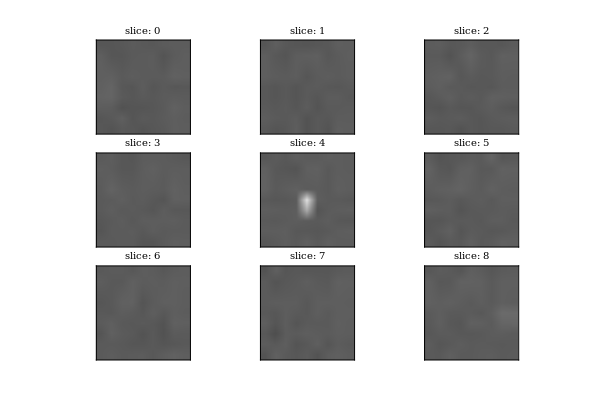
\includegraphics[width=0.66\textwidth]{./Figures/simple_spot_slices.png}
  \caption{Detector image of a single spot across multiple data frames}
  \label{figure: detector spot}
\end{figure}

\begin{figure}
  \centering
  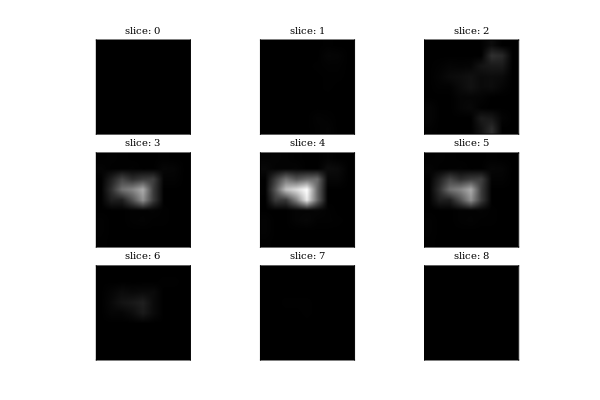
\includegraphics[width=0.66\textwidth]{./Figures/transformed_spot_slices.png}
  \caption{Spot transformed onto the reflection coordinate system grid.}
  \label{figure: transformed spot}
\end{figure}

\begin{figure}
  \centering
  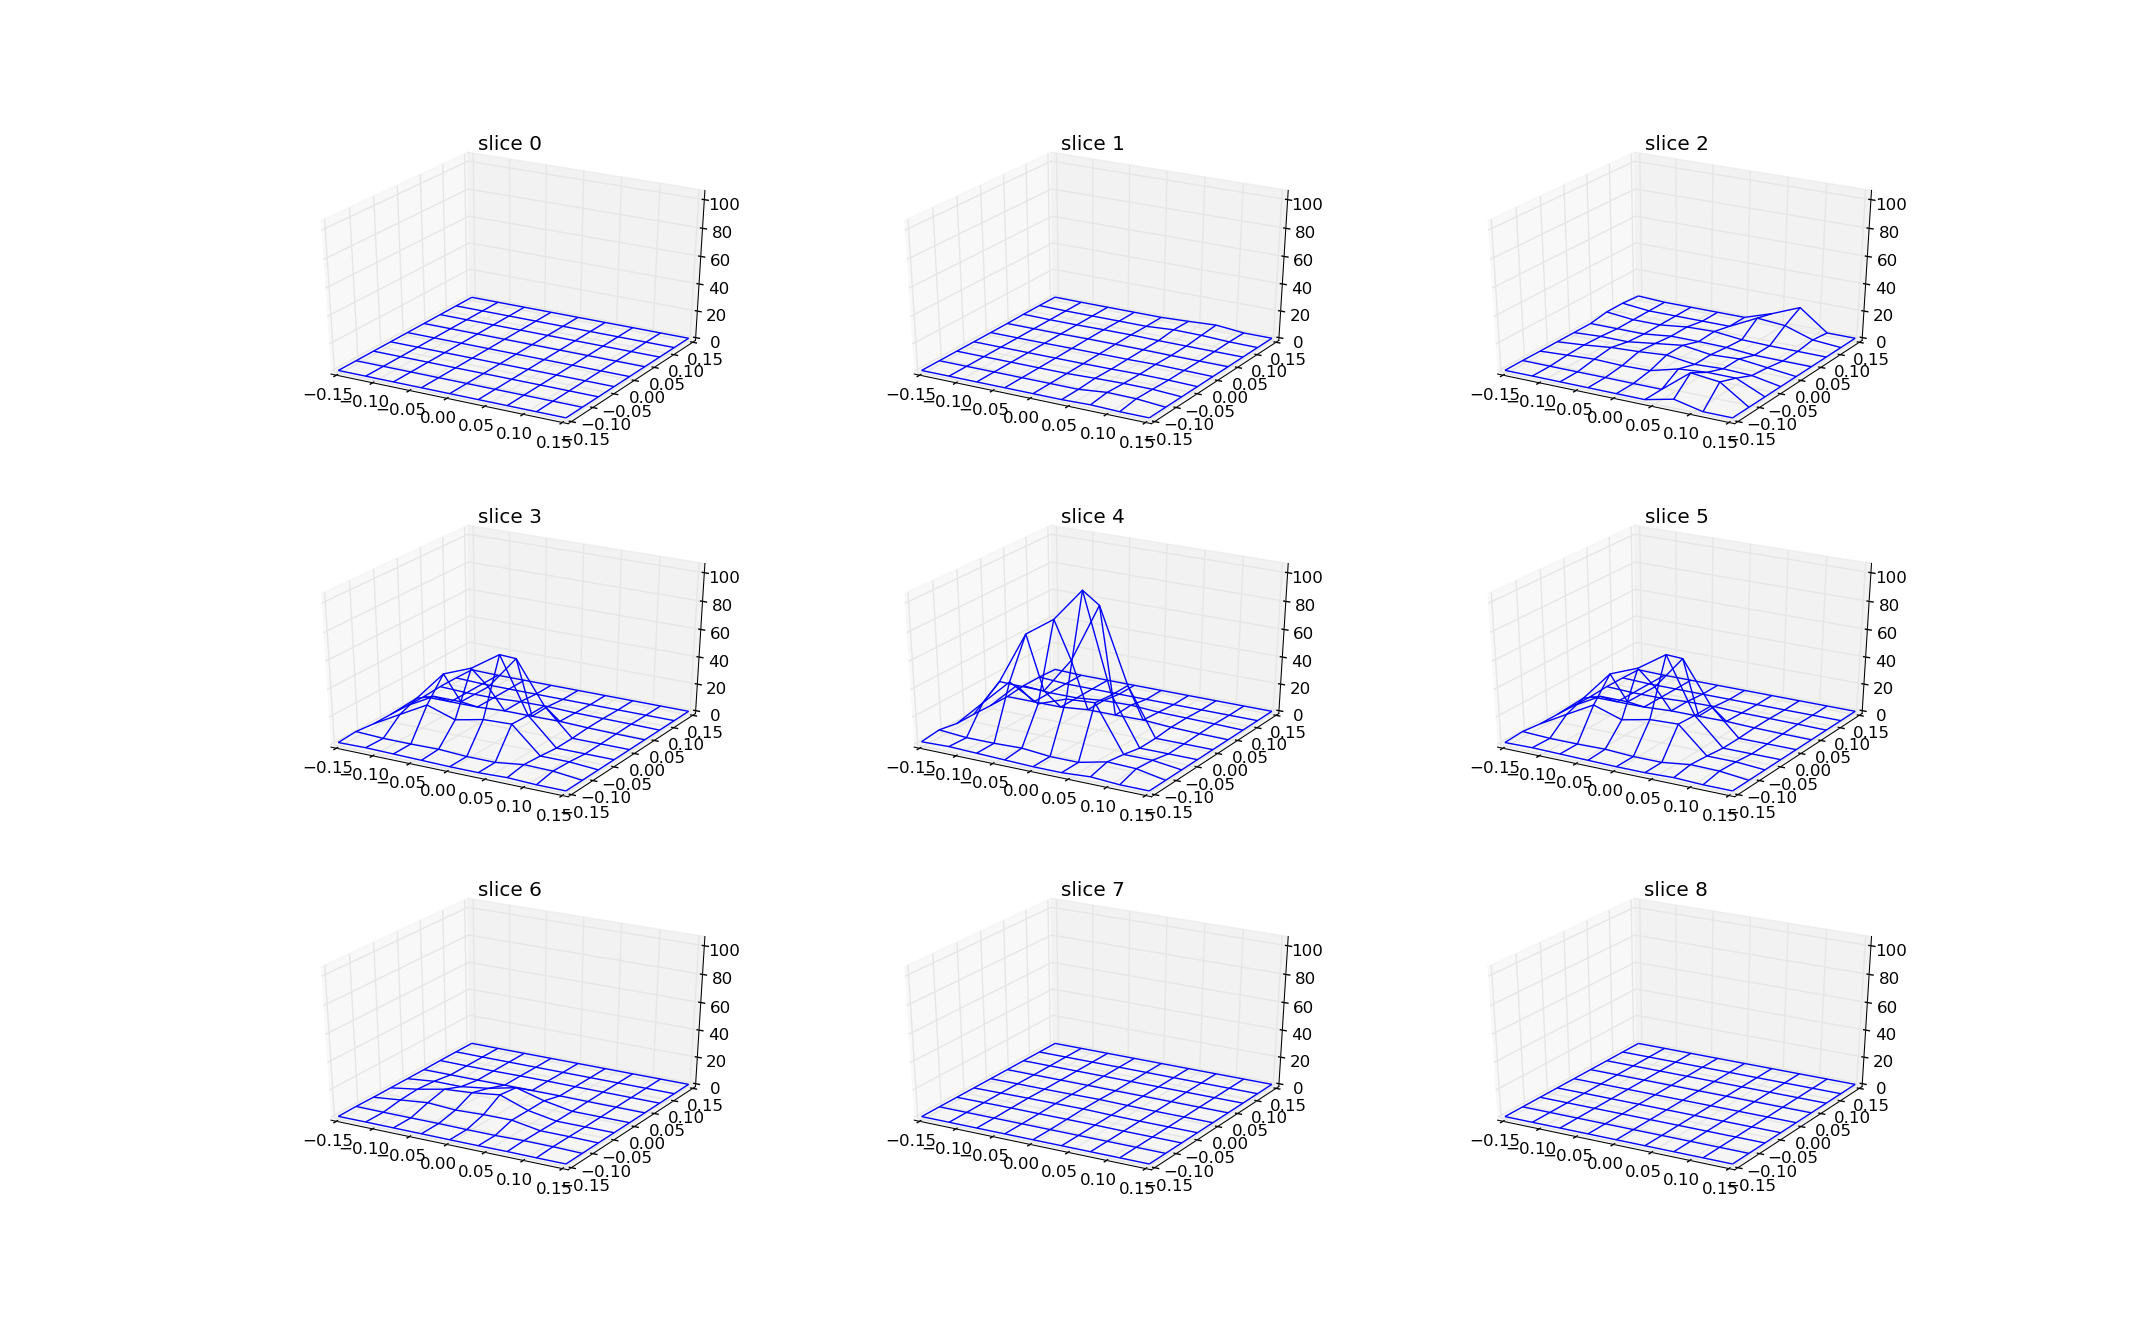
\includegraphics[width=1.00\textwidth]{./Figures/transformed_spot_wireframe.png}
  \caption{Spot transformed onto the reflection coordinate system grid.}
  \label{figure: transformed spot wireframe}
\end{figure}


\end{document}
